\documentclass{article}
\usepackage[utf8]{inputenc}
\usepackage[a4paper, left=2.5cm, right=2.5cm, top=3cm,bottom=3cm]{geometry} %margins
\setcounter{tocdepth}{2}% remove subsubsections from ToC
\usepackage[hidelinks]{hyperref}
\usepackage[nottoc]{tocbibind} %adds references to ToC
\usepackage{afterpage}
\usepackage{amsmath} %do math
\usepackage{mathrsfs} %caligrafic symbols
\usepackage{dutchcal}
\usepackage{amsbsy}
\usepackage{amssymb} % Symbols like \blacktriangledown
\usepackage{stackengine} %Stacking symbols
\usepackage[version=4]{mhchem} %chemical eqations

\usepackage{siunitx} %get SI units
\DeclareSIUnit{\atm}{atm}
\DeclareSIUnit{\angstrom}{\AA}

\usepackage{float} %stuff that floats around
\usepackage{multirow}
\usepackage{booktabs}   %tables and stuff
\usepackage{longtable}
\usepackage{diagbox} %diagonally split cells in tables
\usepackage{graphicx} %extra options when inputting figures
\usepackage{subfig} %subfigures
\usepackage{cleveref} %Reference "Figures 1 to 4 and 5"
\newcommand{\crefrangeconjunction}{-} %Change to display "Figures 1-4 and 5" instead

\usepackage{listings} %add python code to document

\usepackage{enumitem} % for listing stuff (bulletpoints and so on)
\usepackage{setspace} %if you want to change linespacing
\usepackage[parfill]{parskip} %spacing between paragraphs

\usepackage{url} %for references
\usepackage{doi} %for references
\usepackage[super, square, comma, sort&compress]{natbib} %reference package

\numberwithin{equation}{section} %Number eq's by section
\numberwithin{figure}{section} %number figs by section
\numberwithin{table}{section} %number tabels by section

\usepackage{comment} %til blokkommentarer
\usepackage[usenames,dvipsnames]{xcolor}
\usepackage{todonotes}

\usepackage{ifthen} % For if-else statements

\setcounter{MaxMatrixCols}{20}
%Putting self-defined commands here

\renewcommand{\Vec}[1]{\boldsymbol{\mathrm{#1}}} % pretty vectors
\renewcommand{\vec}[1]{\Vec{#1}}
\newcommand{\Mat}[1]{\underline{\pmb{#1}}} % Matrices

% Common symbols
% Fluxes
\newcommand{\bvec}[1]{\Bar{\Vec{#1}}}
\newcommand{\flux}[2]{\Vec{J}_{#1}^{(#2)}}
\newcommand{\mflux}{\Vec{J}^{(n,m)}}
\newcommand{\qflux}{\Vec{J}_q}

% Thermo
% Vectors
\newcommand{\vx}{\vec{x}}
\newcommand{\vn}{\vec{n}}

\newcommand{\Lmm}{L_{\mu \mu}}
\newcommand{\Lmq}{L_{\mu q}}
\newcommand{\Lqm}{L_{q \mu}}
\newcommand{\Lqq}{L_{qq}}

\newcommand{\ST}{S_{T,1}}
\newcommand{\Kr}{K_{\rho}}
\newcommand{\Arho}{A_{\rho}}
\newcommand{\Brho}{B_{\rho}}

\newcommand{\Ta}{T^{\alpha}}
\newcommand{\Tb}{T^{\beta}}
\newcommand{\Va}{V^{\alpha}}
\newcommand{\Vb}{V^{\beta}}
\newcommand{\na}{n^{\alpha}}
\newcommand{\nb}{n^{\beta}}
\newcommand{\xa}{x^{\alpha}}
\newcommand{\xb}{x^{\beta}}
\newcommand{\vna}{\vn^{\alpha}}
\newcommand{\vnb}{\vn^{\beta}}
\newcommand{\vxa}{\vx^{\alpha}}
\newcommand{\vxb}{\vx^{\beta}}


% Kinetic gas theory
\newcommand{\vr}{\vec{r}}
\newcommand{\vu}{\vec{u}}
\newcommand{\bvu}{\Bar{\vec{u}}}
\newcommand{\cvel}[1]{\bvec{u}_{#1}}
\newcommand{\vU}{\vec{U}}
\newcommand{\cVel}{\bvec{U}}
\newcommand{\sD}{\mathscr{D}}
\newcommand{\sU}{\mathscr{U}}
\newcommand{\vsU}{\pmb{\mathscr{U}}}
\newcommand{\vA}{\vec{\Lambda}}
\newcommand{\tvA}{\Tilde{\vA}}
\newcommand{\vD}{\vec{D}}
\newcommand{\vd}{\vec{d}}
\newcommand{\mB}{\Mat{B}}
\newcommand{\va}{\vec{a}}
\newcommand{\sg}{\mathcal{g}}
\renewcommand{\d}{\mathrm{d}}
\newcommand{\rdf}{\Tilde{\chi}}

% Differentials
\renewcommand{\d}{\mathrm{d}}
\newcommand{\dT}{\d T}
\newcommand{\dV}{\d V}
\newcommand{\drho}{\d \rho}
\newcommand{\dr}{\d r}
\newcommand{\dn}{\d n}
\newcommand{\dx}{\d x}
\newcommand{\dA}{\d A}
\newcommand{\dmu}{\d\mu}

% Finite differences
\newcommand{\Dn}{\Delta n}
\newcommand{\Dx}{\Delta x}
\newcommand{\DT}{\Delta T}

\newcommand{\symbline}[3]{$ #1 $ & #2 & \si{#3} \\} % quick symbol table: \symbline{symbol}{description}{unit}
\newcommand{\abrline}[2]{#1 & #2 \\} % Abbreviation & Description
\newcommand{\subline}[2]{$#1$ & #2} % Subscript & Description
%%%%%%%%%%%%%%%%%%%%%%%%%%%%%%%%%%%%%%%%%%%%%%%%%%%%%%%%%%%%%%%%%%%%%%%%%%%%%%%%%%%%%%%%%%%%%%%%%%%%%%%%%%%%
%       quick maffs       %
\newcommand{\del}{\partial} 
\newcommand{\pfrac}[2]{\left(\frac{#1}{#2}\right)} %fraction with parentheses around
\newcommand{\pder}[2]{\frac{\del #1}{\del #2}} %partial derivative of x with respect to y as \pder{x}{y}
\newcommand{\ppder}[2]{\left(\pder{#1}{#2}\right)} %\pder{}{} but with parentheses
\newcommand{\der}[2]{\pfrac{\d #1}{\d #2}}
\newcommand{\lrp}{\left(}
\newcommand{\rrp}{\right)}
\newcommand{\lsp}{\left[}
\newcommand{\rsp}{\right]}
\newcommand{\lcp}{\left\{}
\newcommand{\rcp}{\right\}}
\newcommand{\DeltaAB}{\underset{\alpha,\beta}{\Delta}}
\newcommand{\DeltaIG}{\underset{ig}{\Delta}}
\newcommand{\DeltaHS}{\underset{HS}{\Delta}}
\newcommand{\stackmax}[1]{\stackanchor{$\max$}{\tiny{$#1$}}}

\newcommand{\spder}[3]{
  \ifthenelse{\equal{\detokenize{#2}}{\detokenize{#3}}}
    {\left(\frac{\del^2 #1}{\del #2^2}\right)}
    {\left(\frac{\del^2 #1}{\del #2 \del #3}\right)}%
}

\newcommand{\abs}[1]{\left|#1\right|}
\newcommand{\mathsec}[1]{\texorpdfstring{#1}{TEXT}}
\title{Binary limits of ternary systems}
\author{Vegard Gjeldvik Jervell}

\begin{document}

\maketitle
\tableofcontents

\section{Introduction}

This memo discusses the binary limit of diffusion- and thermal diffusion coefficients in ternary systems, i.e. the behaviour of the coefficients when the mole fraction of one species in the system approaches zero. As an initial remark, please note that if one of the mole fractions is exactly zero, the solutions to Eq. (6), (8) and (10) in \cite{retmie} are ill-defined, such that we cannot model a binary system as a ternary system where one mole fraction is exactly zero. We can, however, investigate the behaviour when one mole fraction approaches zero.

The purpose of this memo is to give some insight into which ternary coefficients approach various binary coefficients in the binary limit, as well as showing how the formulation of the force-flux relations in the respective binary and ternary systems effects these relations.

Finally, the current memo serves as a consistency check for the ternary coefficients computed using the KineticGas package.

\section{Diffusion}
This section discusses the binary limit of the diffusion coefficients in a ternary system. The purpose of the section is to give insight into how the force-flux in a binary system relate to those in a ternary, how to interpret the diffusion coefficients in a ternary system, and raise awareness regarding potential pitfalls when attempting to model a ternary system as a pseudo-binary system.

\subsection{Notation}\label{sec:diffusion_notation}

In the following text, $D_{ii}^{(b)}$ is used to denote the diffusion coefficient of a binary system, where component $i$ is the independent component. $D_{ii}^{(k)}$ denotes the diagonal elements of the Fick diffusion matrix in a ternary system, where component $k$ is the dependent component. $D_{ij}$ denotes the non-diagonal elements of the Fick diffusion matrix in a ternary system, where components $i$ and $j$ are the independent components.

In section \ref{sec:dependent}, $\tilde{D}_{ij}^{(t)}$ and $\tilde{D}_{ij}^{(b)}$ are used to denote the diffusion coefficients corresponding to the linearly dependent formulations of Fick's law.

\subsection{Independent Fluxes}\label{sec:diff_indep}

For a ternary system (1, 2, 3), we can formulate Fick's law for a set of independent fluxes as either

\begin{equation}
    \begin{split}
        \begin{pmatrix}J_1 \\ J_2\end{pmatrix} = \begin{bmatrix}D_{11}^{(3)} & D_{12} \\ D_{21} & D_{22}^{(3)}\end{bmatrix} \begin{pmatrix}\nabla c_1 \\ \nabla c_2\end{pmatrix},
    \end{split}
    \label{eq:tern_dep3}
\end{equation}
\begin{equation}
    \begin{split}
        \begin{pmatrix}J_1 \\ J_3\end{pmatrix} = \begin{bmatrix}D_{11}^{(2)} & D_{13} \\ D_{31} & D_{33}^{(2)}\end{bmatrix} \begin{pmatrix}\nabla c_1 \\ \nabla c_3\end{pmatrix},
    \end{split}
    \label{eq:tern_dep2}
\end{equation}
or
\begin{equation}
    \begin{split}
        \begin{pmatrix}J_2 \\ J_3\end{pmatrix} = \begin{bmatrix}D_{22}^{(1)} & D_{23} \\ D_{32} & D_{33}^{(1)}\end{bmatrix} \begin{pmatrix} \nabla c_2 \\ \nabla c_3\end{pmatrix}.
    \end{split}
    \label{eq:tern_dep1}
\end{equation}
Where the superscript on the diffusion coefficients indicates which component is the dependent component.

For a binary system (1, 2), we can choose between
\begin{equation}
    J_1^{(b)} = D_{11}^{(b)} \nabla c_1
    \label{eq:bin_dep2}
\end{equation}
and
\begin{equation}
    J_2^{(b)} = D_{22}^{(b)} \nabla c_2.
    \label{eq:bin_dep1}
\end{equation}

Now we can examine the question: "When $x_3 \to 0$, and (necessarily) $\nabla c_3 \to 0$ and $J_3 \to 0$, do the ternary coefficients reduce to the corresponding binary coefficients?"

To answer that question, we must be clear about which ternary formulation reduces to which binary formulation.

In the ternary formulation \eqref{eq:tern_dep2}, $J_2$ is the dependent flux, so if $x_3 = \nabla c_3 = 0$ (something we are free to demand, as $\nabla c_1$ and $\nabla c_3$ are independent), $J_1 = D_{11}^{(2)} \nabla c_1$. Thus, we expect that formulation \eqref{eq:tern_dep2} should reduce to formulation \eqref{eq:bin_dep2} when $x_3 = \nabla c_3 = 0$. Therefore, we expect
\begin{equation}
    D_{11}^{(2)}(x_3 = 0) = D_{11}^{(b)}.
\end{equation}

By similar argument, it's formulation \eqref{eq:tern_dep1} that reduces to formulation \eqref{eq:bin_dep1}, so
\begin{equation}
    D_{22}^{(1)}(x_3 = 0) = D_{22}^{(b)}.
\end{equation}

Note that formulation \eqref{eq:tern_dep3} does not immediately reduce to one of the binary formulations when $x_3 \to 0$; this is because in this formulation, we cannot demand $\nabla c_3 = 0$ because component 3 is the dependent component in this formulation. Therefore, the coefficients in formulation \eqref{eq:tern_dep3} cannot be expected to reduce to the binary coefficients when $x_3 \to 0$.

Figure \ref{fig:binary_ternary} shows how the ternary coefficients expected to reduce to the corresponding binary coefficients behave as a function of $x_3$.

\begin{figure}[htb]
    \centering
    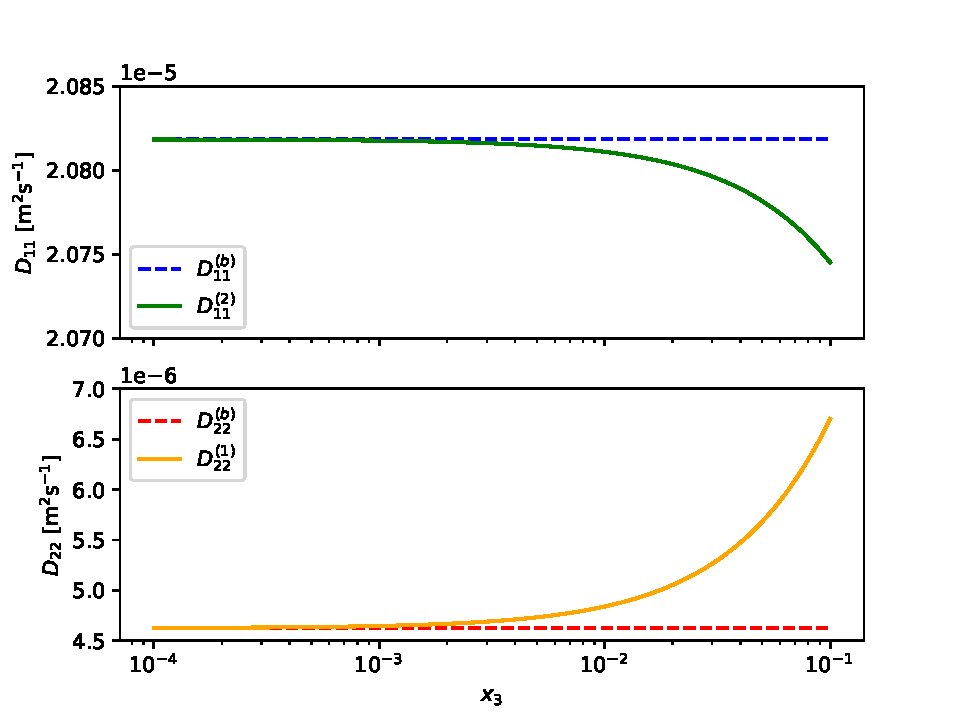
\includegraphics[width=.75\textwidth]{binary_ternary.pdf}
    \caption{The ternary diffusion coefficients reduce to the corresponding binary coefficients when $x_3 \to 0$.}
    \label{fig:binary_ternary}
\end{figure}


\subsection{Dependent Fluxes}\label{sec:dependent}

An alternative flux-force formulation for the ternary system is through a set of \textit{dependent} fluxes and forces; thus, we can formulate Fick's law as

\begin{equation}
    \begin{split}
        \begin{pmatrix}J_1 \\ J_2 \\ J_3 \end{pmatrix} = \begin{bmatrix}\tilde{D}_{11}^{(t)} & \tilde{D}_{12}^{(t)} & \tilde{D}_{13}^{(t)} \\ \tilde{D}_{21}^{(t)} & \tilde{D}_{22}^{(t)} & \tilde{D}_{23}^{(t)} \\ \tilde{D}_{31}^{(t)} & \tilde{D}_{32}^{(t)} & \tilde{D}_{33}^{(t)} \end{bmatrix} \begin{pmatrix}\nabla c_1 \\ \nabla c_2 \\ \nabla c_3\end{pmatrix},
    \end{split}
\end{equation}
and correspondingly for the binary system:
\begin{equation}
    \begin{split}
        \begin{pmatrix}J_1 \\ J_2\end{pmatrix} = \begin{bmatrix}\tilde{D}_{11}^{(b)} & \tilde{D}_{12}^{(b)} \\ \tilde{D}_{21}^{(b)} & \tilde{D}_{22}^{(b)}\end{bmatrix} \begin{pmatrix}\nabla c_1 \\ \nabla c_2\end{pmatrix}.
    \end{split}
\end{equation}

Note that these two matrices are not invertible because they implicitly contain the dependency $J_1 + J_2 + J_3 = 0$. However, this formulation can be useful for consistency checking because when $x_3 \to 0$, Equation \eqref{eq:dep_matr_eqiv} should hold:

\begin{equation}
    \begin{bmatrix}\tilde{D}_{11}^{(t)} & \tilde{D}_{12}^{(t)} \\ \tilde{D}_{21}^{(t)} & \tilde{D}_{22}^{(t)} \end{bmatrix} = \begin{bmatrix}\tilde{D}_{11}^{(b)} & \tilde{D}_{12}^{(b)} \\ \tilde{D}_{21}^{(b)} & \tilde{D}_{22}^{(b)}\end{bmatrix}.
    \label{eq:dep_matr_eqiv}
\end{equation}

This equality should hold precisely because the matrices contain the dependence between the fluxes and forces, and when $x_3 = \nabla c_3 = 0$, $J_1 + J_2 = 0$, and we should obtain the same fluxes as from the binary matrix.

Figure \ref{fig:dependent} demonstrates that Equation \eqref{eq:dep_matr_eqiv} is satisfied when $x_3 \to 0$.

\begin{figure}[bht]
    \centering
    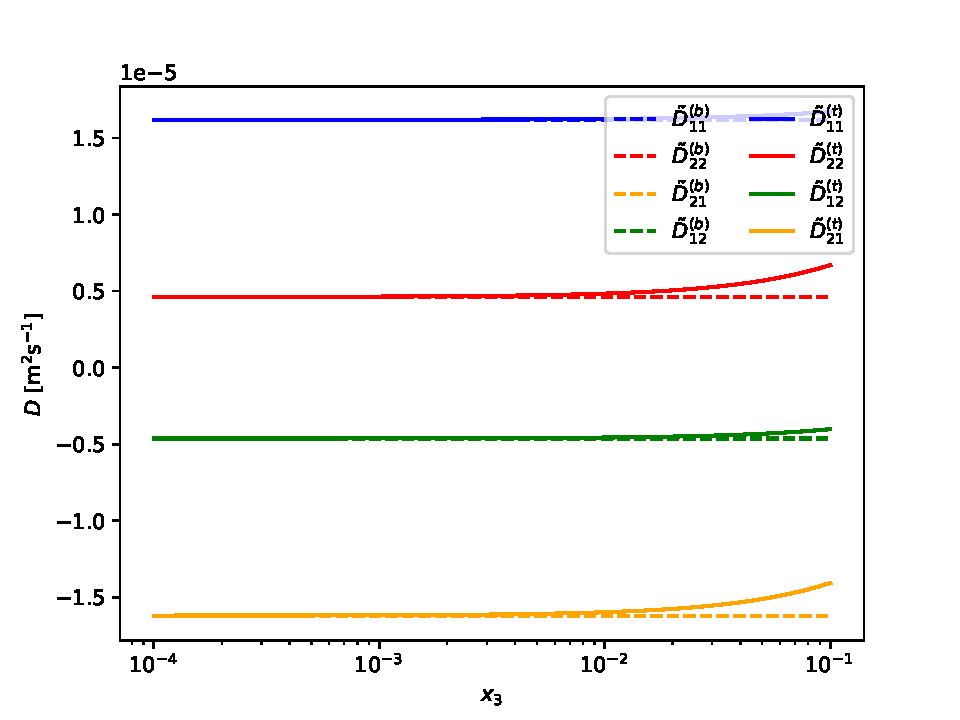
\includegraphics[width=.75\textwidth]{dependent.pdf}
    \caption{The coefficients in the singular, ternary Fick matrix reduce to the corresponding coefficients in the singular, binary Fick matrix when $x_3 \to 0$.}
    \label{fig:dependent}
\end{figure}

Finally, for the ternary matrix, we can observe that
\begin{equation}
    \tilde{D}_{13} - \tilde{D}_{23} = 0
\end{equation}
when $x_3 = 0$ because when $x_3 = \nabla c_3 = 0$, $\nabla c_2 = - \nabla c_1$, and $J_3$ should vanish. Figure \ref{fig:vanish3} demonstrates that this condition is met.

\begin{figure}[bth]
    \centering
    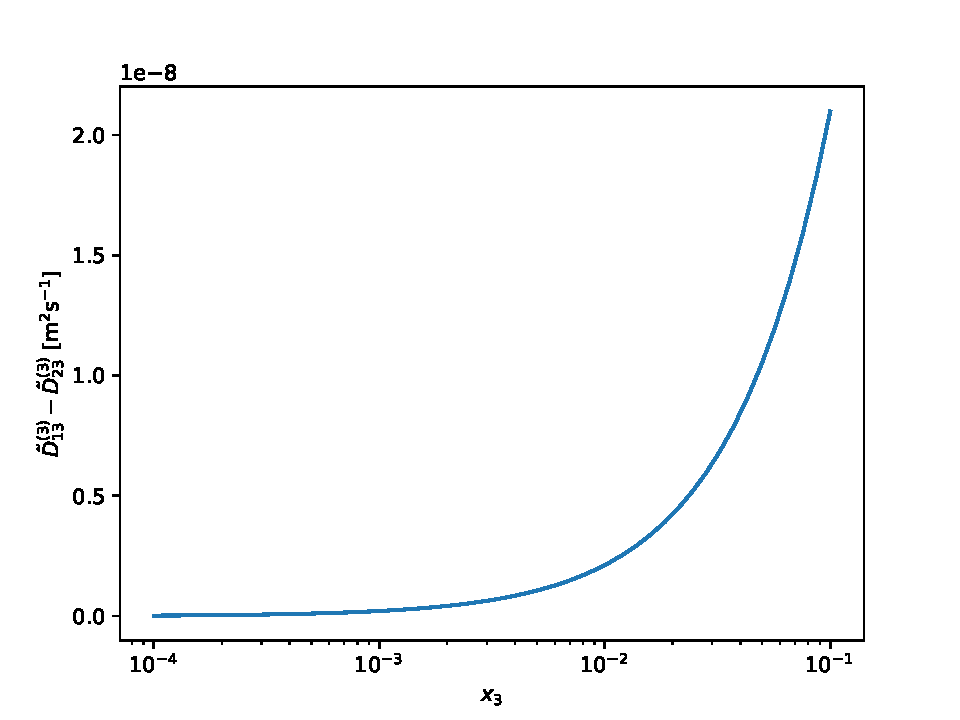
\includegraphics[width=.75\textwidth]{vanish3.pdf}
    \caption{The flux $J_3$ vanishes when $x_3 \to 0$ and $\nabla c_3 = 0$.}
    \label{fig:vanish3}
\end{figure}

\clearpage
\section{Thermal Diffusion}

Thermal diffusion coefficients are defined through an extension of the equations in Sec. \ref{sec:diffusion}, using the same notation as is present there, thermal diffusion coefficients computed using the KineticGas package are defined through
\begin{equation}
    \begin{pmatrix}J_1 \\ J_2 \\ \vdots \\ J_N \end{pmatrix}^{(n, f)} = 
    \begin{pmatrix}
    D_{T,1} \\ D_{T,2} \\ \vdots \\ D_{T,N}    
    \end{pmatrix}^{(f, l)} \nabla \ln T -
    \begin{bmatrix}
    D_{11} & D_{12} & \hdots & D_{1N} \\
    D_{21} & D_{22} & \hdots & D_{2N} \\
    \vdots & \vdots & \ddots & \vdots \\
    D_{N1} & D_{N2} & \hdots & D_{NN}
    \end{bmatrix}^{(f, l)}
    \begin{pmatrix}\nabla c_1 \\ \nabla c_2 \\ \vdots \\ \nabla c_N \end{pmatrix}
    \label{eq:thdiff_definition}
\end{equation}
or, more compactly
\begin{equation}
    \Vec{J}^{(n, f)} = \Vec{D}_T^{(f, l)} \nabla \ln T - \Mat{D}^{(f, l)} \nabla \Vec{c}.
\end{equation}

Note that because in the presence of a temperature gradient, the Gibbs-Duhem equation no longer reduces to 
\begin{equation}
    \sum_i x_i \nabla \mu_i = 0,
\end{equation}
the choice of dependent component ($l$) will not only effect the diffusion matrix $\Mat{D}^{(f, l)}$, but also the thermal diffusion vector $\Vec{D}_T^{(f, l)}$. Just as for the diffusion matrix, the frame of reference and choice of dependent component for thermal diffusion coefficients is selected with the options \code{frame\_of\_reference} and \code{dependent\_idx}, with the \code{thermal\_diffusion\_coeff} method. 

Also, just as for the diffusion matrix, thermal diffusion coefficients computed using the KineticGas package are defined through Eq. \eqref{eq:thdiff_definition}, i.e. with $\nabla \ln T$ and the \textit{molar concentration gradients} as the driving forces, and with the fluxes on a \textit{molar} basis.
\section{Soret coefficients}

The Soret coefficient is a measure of the steady state separation in a mixture induced by a temperature gradient. Ortiz de Zárate \cite{ortiz2019definition} defines the Soret coefficients of a multicomponent mixture ($s$ components) through
\begin{equation}
    \begin{bmatrix}
        x_1 (1 - x1) & x_1 x_2 & \hdots & x_1 x_{s - 1} \\
        x_2 x_1 & x_2 (1 - x_2) & \hdots & x_2 x_{s - 1} \\
        \vdots & & \ddots & \vdots \\
        x_{s - 1} x_1 & & & x_{s - 1}(1 - x_{s - 1}) 
    \end{bmatrix}
    \begin{pmatrix}
        S_{T, 1} \\
        S_{T, 2} \\
        \vdots \\
        S_{T, s - 1}
    \end{pmatrix}
    = 
    - \frac{1}{\nabla T}
    \begin{pmatrix}
        \nabla x_1 \\
        \nabla x_2 \\
        \vdots \\
        \nabla x_{s - 1}
    \end{pmatrix},
\end{equation}
or more compactly,
\begin{equation}
    \Mat{X} \Vec{S}_T = - \frac{\nabla \Vec{x}}{\nabla T}.
\end{equation}
Similarly to the thermal diffusion coefficients, this definition carries the advantage that 
\begin{equation}
    \Mat{X} \Vec{S}_T = - \frac{\nabla \Vec{x}}{\nabla T} \quad \iff \quad \Mat{W} \Vec{S}_T = - \frac{\nabla \Vec{w}}{\nabla T},
\end{equation}
such that mole- and mass fractions can be used interchangably with the same Soret coefficients.

In the state with vanishing mass fluxes ($\Vec{J} = \Vec{0}$). From the condition of vanishing mass fluxes, we find that we can compute the Soret coefficients as\footnote{See the memo on definitions of the diffusion coefficient for notes on $\Mat{D}^{(z)}$.}
\begin{equation}
    \begin{split}
        \Vec{J} = - c \left( \Mat{X} \Vec{D}_{T}^{(z)} \nabla T + \Mat{X} \Mat{D}^{(z)} \Mat{X}^{-1} \nabla \Vec{x} \right) &= \Vec{0} \\
        - \frac{\nabla \Vec{x}}{\nabla T} &= \Mat{X} \left(\Mat{D}^{(z)}\right)^{-1}  \Vec{D}_{T}^{(z)} \\
        \Vec{S}_T &= \left(\Mat{D}^{(z)}\right)^{-1}  \Vec{D}_{T}^{(z)}.
    \end{split}
\end{equation}

For a binary system (1, 2), this definition thus yields
\begin{equation}
    S_{T, 1}^{(b)} = \frac{D_{T, 1}^{(z, b)}}{D_{11}^{(z, b)}}.
\end{equation}

From the preceding relations it is possible to show that when using this definition of the Soret coefficient \cite{ortiz2019definition},
\begin{equation}
    \begin{split}
        \lim_{x_1 \to 0} S_{T, 2} = S_{T, 2}^{(b, 3)} \\
        \lim_{x_2 \to 0} S_{T, 1} = S_{T, 1}^{(b, 3)} \\
        \lim_{x_3 \to 0} S_{T, 1} - S_{T, 2} = S_{T, 1}^{(b, 2)},
    \end{split}
    \label{eq:soret_binary_limit}
\end{equation}
where $S_{T, i}^{b, j}$ denotes the Soret coefficient of component $i$ in a binary mixture with $j$, with species $j$ being the dependent species. Figure \ref{fig:soret_binary_limit} shows how this convergence behaviour is obeyed.

\begin{figure}
    \centering
    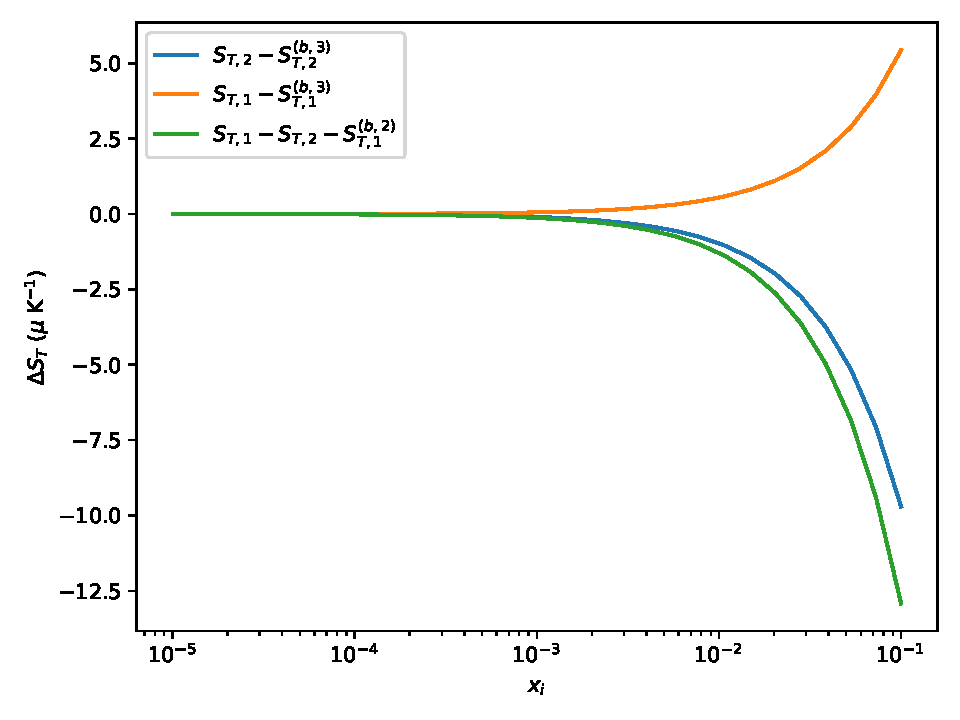
\includegraphics[width=.85\textwidth]{soret_limit.pdf}
    \caption{The convergence of the ternary Soret coefficient to the corresponding binaries as indicated in Eq. \eqref{eq:soret_binary_limit}.}
    \label{fig:soret_binary_limit}
\end{figure}

\clearpage

\bibliographystyle{ieeetr}
\bibliography{bibliografi}

\end{document}
